\documentclass[a4 paper]{article}
% Set target color model to RGB



\usepackage[inner=2.0cm,outer=2.0cm,top=2.5cm,bottom=2.5cm]{geometry}
\usepackage{setspace}
\usepackage[rgb]{xcolor}
\usepackage{verbatim}
\usepackage{subcaption}
\usepackage{amsgen,amsmath,amstext,amsbsy,amsopn,tikz,amssymb,tkz-linknodes}
\usepackage{fancyhdr}
\usepackage[colorlinks=true, urlcolor=blue,  linkcolor=blue, citecolor=blue]{hyperref}
\usepackage[colorinlistoftodos]{todonotes}
\usepackage{rotating}
%\usetikzlibrary{through,backgrounds}

\usepackage{lmodern}
\usepackage[T1]{fontenc}
\usepackage[capposition=top]{floatrow}
\usepackage{hyperref}
\usepackage{graphicx}
\graphicspath{ {images/} }
\usepackage{booktabs}
\usepackage{changepage}
\usepackage{float}








\hypersetup{%
pdfauthor={Nick Korbit},%
pdftitle={Homework},%
%pdfkeywords={Tikz,latex,bootstrap,uncertaintes},%
pdfcreator={PDFLaTeX},%
pdfproducer={PDFLaTeX},%
}
%\usetikzlibrary{shadows}
% \usepackage[francais]{babel}
\usepackage{booktabs}


\newcommand{\ra}[1]{\renewcommand{\arraystretch}{#1}}

\newtheorem{thm}{Theorem}[section]
\newtheorem{prop}[thm]{Proposition}
\newtheorem{lem}[thm]{Lemma}
\newtheorem{cor}[thm]{Corollary}
\newtheorem{defn}[thm]{Definition}
\newtheorem{rem}[thm]{Remark}
\numberwithin{equation}{section}

\newcommand{\homework}[6]{
   \pagestyle{myheadings}
   \thispagestyle{plain}
   \newpage
   \setcounter{page}{1}
   \noindent
   \begin{center}
   \framebox{
      \vbox{\vspace{2mm}
    \hbox to 6.28in { {\bf ISYE 6420:~Bayesian Statistics \hfill {\small #2}} }
       \vspace{6mm}
       \hbox to 6.28in { {\Large \hfill #1  \hfill} }
       \vspace{6mm}
       \hbox to 6.28in { {\it Instructor: {\rm #3} \hfill Name: {\rm #5}, gtID: {\rm #6}} }
       %\hbox to 6.28in { {\it TA: #4  \hfill #6}}
      \vspace{2mm}}
   }
   \end{center}
   \markboth{#5 -- #1}{#5 -- #1}
   \vspace*{4mm}
}

\newcommand{\problem}[2]{~\\\fbox{\textbf{Problem #1}}\newline\newline}
\newcommand{\subproblem}[1]{~\newline\textbf{(#1)}}
\newcommand{\D}{\mathcal{D}}
\newcommand{\Hy}{\mathcal{H}}
\newcommand{\VS}{\textrm{VS}}
\newcommand{\solution}{~\newline\textbf{\textit{(Solution)}} }

\newcommand{\bbF}{\mathbb{F}}
\newcommand{\bbX}{\mathbb{X}}
\newcommand{\bI}{\mathbf{I}}
\newcommand{\bX}{\mathbf{X}}
\newcommand{\bY}{\mathbf{Y}}
\newcommand{\bepsilon}{\boldsymbol{\epsilon}}
\newcommand{\balpha}{\boldsymbol{\alpha}}
\newcommand{\bbeta}{\boldsymbol{\beta}}
\newcommand{\0}{\mathbf{0}}



%%%%%%%%%%%%%%%%%%%%%%%%%%%%%%%%%%%%%%%%
%%			 Document				  %%
%%%%%%%%%%%%%%%%%%%%%%%%%%%%%%%%%%%%%%%%


\begin{document}
	
\homework{Homework \#3}{Spring 2020}{Roshan Vengazhiyil, Brani Vidakovic}{}{Nick Korbit}{903263968}


%%%%%%%%%%%%%%%%%%%%%%%%%%%%%%%%%%%%%%%%
%%			 Part I					  %%
%%%%%%%%%%%%%%%%%%%%%%%%%%%%%%%%%%%%%%%%




\problem{1}

\textbf{a$)$.} We first find the probability 
of an individual component to stay alive at time $t$:

$$
p=e^{-0.1 \times t^{3 / 2}}
$$
$$
p=e^{-0.1 \times 3^{3 / 2}} \approx 0.594749
$$

Then we have two options to find the probability 
that a k-out-of-n system is still operational when 
checked at
time $t=3$ ($P^s_3$). First, we can leverage the probability 
mass function and sum up probabilities that 
exactly 4, 5, 6, 7 and 8 components are alive at $t=3$:

$$
\operatorname{Pr}(X=k)=\left(\begin{array}{l}
{n} \\
{k}
\end{array}\right) p^{k}(1-p)^{n-k}
$$

For $n=8$, $k=4$, $p=0.594749$ we have:

$$
P_{3}^{s}=Pr(X=4)+Pr(X=5)+Pr(X=6)+Pr(X=7)+Pr(X=8)
$$

$$
P_{3}^{s} \approx 0.818094
$$


We can also utilize the cumulative
distribution function. Cdf for binomial distribution is 

$$
F(k ; n, p)=\operatorname{Pr}(X \leq k)=\sum_{i=0}^{|k|}\left(\begin{array}{l}
{n} \\
{i}
\end{array}\right) p^{i}(1-p)^{n-i}
$$

In order to evaluate the system staying alive at $t=3$ 
we need to compute 

$$
P_{3}^{s} = 1 - F(3; 8, p)
$$

So that 

$$
P_{3}^{s} \approx 0.818094
$$

Confirming our previous result. \newline



\textbf{b$)$.} Let's apply the Bayes formula to find
the probability that at time $t=3$ exactly 5 components 
were operational (event $X$) given the system was found 
operational (event $H$):

$$
P(X|H)=\frac{P(H|X)P(X)}{P(H)}
$$

If 5 components are operational, then the system is 100\% 
alive, so that $P(H|X)$ is a sure event, $P(H|X)=1$.
We have already calculated $P(H)$, it's basically $P_{3}^{s}$.  
And $P(X)$ can be calculated as $\operatorname{Pr}(X=5)$:

$$
P(X) = pmf(5, 8, 0.594749) \approx 0.277351
$$

Then $P(X|H)$ is
$$
P(X|H) = 0.277351/0.818094 \approx 0.339021
$$ \newline


Note. The script for solving Q1 is implemented in 
\textit{hw2q2.py}, function \textit{solve\_q1()} 
(included in the zip archive). To run the code just run 
\textit{'python hw2q2.py'}. 







\problem{2}

\textbf{a$)$.} In order to find 
the probability that a
randomly chosen measurement can be classified as accurate
we need to integrate the pdf on the selected interval $(-0.5,0.5)$.
We utilize the fact that the pdf is symmetrical wrt y-axis:

$$
p=\int_{-0.5}^{0.5}\frac{3x^{2}}{16}dx=2\int_{0}^{0.5}\frac{3x^{2}}{16}dx=2\frac{0.5^{3}}{16}=0.015625
$$

So that the desired probability is about 1.6\%. \newline

\textbf{b$)$.} We now find and plot a cdf. Remember that 
the cdf of a continuous random variable is 

$$
F(x)=\int_{-\infty}^{x} f(t) d t
$$

For our function:

$$
F(x)=\int_{-2}^{x}\frac{3t^{2}}{16}dt=\frac{x^{3}}{16}-\frac{(-2)^{3}}{16}=\frac{x^{3}}{16}+\frac{1}{2}
$$

Let's plot the cdf on the $(-2,2)$ interval:

\begin{figure}[H]
	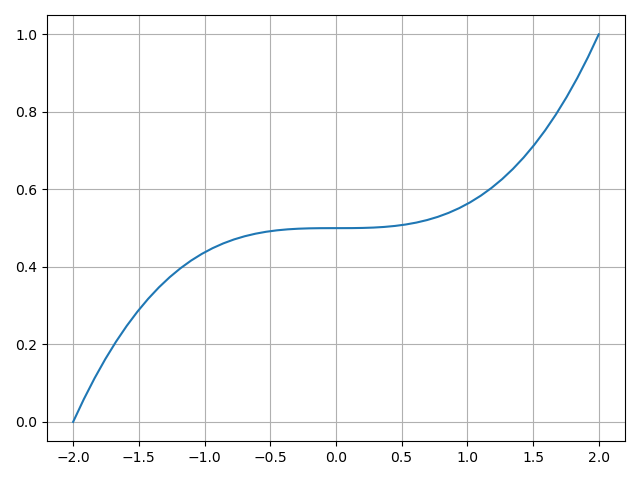
\includegraphics[scale=0.4]{q2cdf}
	\centering
%	\caption{cdf .}
	\label{q2cdf}
\end{figure}

Combining all intervals the cdf is:
$$
F(x)=\begin{cases}
0, & x\leq-2\\
\frac{x^{3}}{16}+\frac{1}{2}, & -2<x<2\\
1, & x\geq2
\end{cases}
$$ \newline



\textbf{c$)$.} Finding $\mathbb{E}[Y]$ in our case
is equivalent to finding a second moment:

$$
\mathrm{E}\left[X^{2}\right]=\int_{-\infty}^{\infty}x^{2} f(x) d x
$$

For our function:

$$
\mathrm{E}\left[X^{2}\right]=\int_{-2}^{2}x^{2} \frac{3x^{2}}{16} d x = 2\int_{0}^{2}\frac{3x^{4}}{16}dx=2(\frac{3\cdot2^{5}}{16\cdot5}-0)=\frac{3\cdot2^{2}}{5}=2.4
$$

So that the expected loss is 2.4 thousands of dollars. \newline


\textbf{d$)$.} To compute the probability that 
the loss is less than $y$ we utilize the cdf of $X$:

$$
P(Y<y)=P(X^{2}<y)=P(-\sqrt{y}<X<\sqrt{y})=\int_{-\sqrt{y}}^{\sqrt{y}}f(x)dx
$$

$$
P(X^{2}<3)=\int_{-\sqrt{3}}^{\sqrt{3}}\frac{3x^{2}}{16}dx=2\int_{0}^{\sqrt{3}}\frac{3x^{2}}{16}dx=\left.2\frac{x^{3}}{16}\right|_{0}^{\sqrt{3}}=\frac{2(\sqrt{3}^{3})}{16}\approx0.649519
$$

So that the probability that the loss is less than 3 
thousand is approximately 65\%. \newline

Note. The script for plotting Q2.B chart is implemented in 
\textit{hw2q2.py}, function \textit{solve\_q2()} 
(included in the zip archive). To run the code just run 
\textit{'python hw2q2.py'}.




\problem{3}

\textbf{a$)$.} We find the marginal distribution $f_X(x)$
by integrating the joint pdf wrt $y$:

$$
f_{X}(x)=\int_{0}^{1}(x+y)dy=x+\left.\frac{y^{2}}{2}\right|_{0}^{1}=x+\frac{1}{2}
$$

Or, more formally,
$$
f_{X}(x)=\begin{cases}
	x+\frac{1}{2}, & 0\leq x\leq1\\
	0, & else
\end{cases}
$$


\textbf{b$)$.} Let's then find the 
conditional distribution $f(y|x)$:
$$
f(y|x)=\frac{f(x,y)}{f(x)}=\frac{x+y}{x+\frac{1}{2}}
$$

Or, more formally,
$$
f(y|x)=\begin{cases}
\frac{x+y}{x+\frac{1}{2}}, & 0\leq x\leq1;0\leq y\leq1\\
0, & else
\end{cases}
$$


\problem{4}

\textbf{a$)$.} Let's apply the Bayes theorem:

$$
\pi(\theta|x)=\frac{f(x|\theta)\pi(\theta)}{m(x)}
$$

The posterior $\pi(\theta|x)$ belongs to the Pareto family:
$$
\pi(\theta|x)=\frac{\alpha c^{\alpha}}{\theta^{\alpha+1}} \mathbf{1}(\theta>c)
$$ 

The prior $\pi(\theta)$ is:
$$
\pi(\theta)=\frac{1}{\theta} \mathbf{1}(\theta>0)
$$

The conditional $f(x|\theta)$ is:
$$
f(x|\theta) = \theta^{-34} \mathbf{1}(\theta>M)
$$

We now calculate the joint probability:
$$
f(x,\theta) = f(x|\theta)\pi(\theta)=\frac{1}{\theta} \mathbf{1}(\theta>0)\theta^{-34} \mathbf{1}(\theta>M) = \theta^{-35} \mathbf{1}(\theta>0)\mathbf{1}(\theta>M) = \theta^{-35}\mathbf{1}(\theta>M)
$$

The marginal $m(x)$ is:
$$
m(x)=\int_{\varTheta}f(x,\theta)d\theta=\int_{M}^{\infty}\theta^{-35}\mathbf{1}(\theta>M)d\theta=\int_{M}^{\infty}\theta^{-35}d\theta=\left.-\frac{1}{34x^{34}}\right|_{M}^{\infty}=0-\left(-\frac{1}{34M^{34}}\right)=\frac{1}{34M^{34}}
$$

Getting back to the Bayes theorem:

$$
\frac{\alpha c^{\alpha}}{\theta^{\alpha+1}} \mathbf{1}(\theta>c) = \frac{\theta^{-35}\mathbf{1}(\theta>M)}{\frac{1}{34M^{34}}}=\frac{34M^{34}}{\theta^{35}}\mathbf{1}(\theta>M)
$$

So that we can derive that $\alpha=34$ and $c=M=0.54876$. \newline


\textbf{b$)$.} As we have a Pareto distribution, we can calculate 
$E[\theta]$:

$$
E[\theta]=\frac{34\cdot0.54876}{34-1}\approx0.565389
$$

We now calculate lower and upper bounds, $L$ and $U$ respectively:
$$
\int_{-\infty}^{L} \pi(\theta | x) d \theta=\alpha / 2
$$
We can substitute the integral with the cdf:
$$
cdf(L) =\alpha / 2
$$

$$
\left[1-(M/L)^{34}\right]\mathbf{1}(L>M)=\frac{\alpha}{2}
$$

$$
L=\frac{M}{\sqrt[34]{1-\frac{\alpha}{2}}}
$$

$$
L=\frac{0.54876}{\sqrt[34]{1-\frac{0.05}{2}}}\approx 0.549169
$$

The upper bound $U$ is:
$$
\int_{-\infty}^{U} \pi(\theta | x) d \theta=1-\alpha / 2
$$
$$
\left[1-(M/U)^{34}\right]\mathbf{1}(U>M)=1-\frac{\alpha}{2}
$$

$$
U=\frac{M}{\sqrt[34]{\frac{\alpha}{2}}}
$$

$$
U=\frac{0.54876}{\sqrt[34]{\frac{0.05}{2}}}\approx 0.611648
$$

So that the $[U;L]$ bounds are $[0.549169;0.611648]$
and $\theta=0.6$ is inside the interval.


%%%%%%%%%%%%%%%%%%%%%%%%%%%%%%%%%%%%%%%%
%%			 Bibliography			  %%
%%%%%%%%%%%%%%%%%%%%%%%%%%%%%%%%%%%%%%%%

\begin{thebibliography}{9}


\bibitem{stat}\label{stat} 
Engineering Biostatistics: An Introduction using MATLAB and WinBUGS. 
Brani Vidakovic - Wiley Series in Probability and Statistics.

\end{thebibliography}



\end{document} 